\section{Efficiency Evaluation \& Simulations}
  \label{section:comparison}
  We offer here a cost and efficiency comparison of this work with
  LVPC~\cite{10.1007/978-3-030-65411-5_18} and Donner~\cite{donner}. We focus on
  these due to their exclusive support of
  virtual channels over any number of base channels. We remind that LVPC
  achieves this via recursion, while Donner
  because it is variadic (cf. Table~\ref{table:comparison-features}).

  We count the communication, storage and on-chain cost of a virtual
  channel in each protocol. We also simulate the execution of a large number
  of payments among many parties and derive payment latency and fees -- contrary
  to our theoretical analysis, fees are included in our simulations to make the
  comparison more robust. We thus
  obtain an end-to-end understanding of both the requirements and benefits
  of each protocol.

  \makeatletter%
  \@ifclassloaded{IEEEtran}%
    {\paragraph{Cost calculation}}%
    {\paragraph{Cost calculation.}}%
  \makeatother%
  Consider the setting of $1$
  funder ($P_1$), $1$ fundee ($P_n$) and $n-2$ intermediaries ($P_2, \dots,
  P_{n-1}$) where $P_i$ has a base channel with each of $P_{i-1}$,
  $P_{i+1}$. We compare the costs of off-chain opening
  (Table~\ref{table:comparison:overhead:n-parties:open}) and on-chain
  closing unilaterally
  (Table~\ref{table:comparison:overhead:n-parties:close}).
  % splncs
  %See Appx.~\ref{section:cost-details} for comparison details and choices.

  Regarding opening, in
  Table~\ref{table:comparison:overhead:n-parties:open} we calculate for each of
  the $3$ protocols the number of communication rounds required, the total
  size of outgoing messages as well as the amount of space for storing
  channel data. We calculate funder, fundee
  and intermediary requirements, along with the aggregate for all parties.
  % acmart
  The communication rounds for a party are calculated as its [\#incoming
  messages + \#outgoing messages]/2. The size of outgoing messages and the
  stored data are measured in raw bytes. The data is counted as the sum of the
  relevant channel identifiers ($8$ bytes each, as defined by the Lightning
  Network
  specification\footnote{\url{https://github.com/lightning/bolts/blob/master/07-routing-gossip.md\#definition-of-short_channel_id}}),
  transaction output identifiers ($36$ bytes), secret keys ($32$ bytes each),
  public keys ($32$ bytes each, compressed form -- these double as party
  identifiers), Schnorr signatures ($64$ bytes each), coins ($8$ bytes each),
  times and timelocks (both $4$ bytes each). UC-specific data is ignored.

  For LVPC, multiple different topologies can support a virtual channel between
  $P_1$ and $P_n$ (all of which need $n-1$ base channels). We here consider the
  case in which the funder $P_1$ first opens one virtual channel with $P_3$ on
  top of channels $(P_1, P_2)$ and $(P_2, P_3)$, then another virtual channel
  with $P_4$ over $(P_1, P_3)$ and $(P_3, P_4)$ and so on up to the $(P_1, P_n)$
  channel, opened over $(P_1, P_{n-1})$ and $(P_{n-1}, P_n)$. We choose this
  topology as $P_1$ cannot assume that there exist any virtual channels between
  other parties (which could be used as shortcuts).

  A subtle byproduct of the above topology is that during the opening phase of
  LVPC every intermediary $P_i$ acts both as a fundee in its virtual channel
  with the funder $P_1$ and as an intermediary in the virtual channel of $P_1$
  with the next party $P_{i+1}$. The above does not apply to the first
  intermediary $P_2$, since it already has a channel with $P_1$ before the
  protocol starts. Table~\ref{table:comparison:overhead:n-parties:open} shows
  the total cost of intermediaries $P_3, \dots, P_{n-1}$. The first intermediary
  $P_2$ incurs instead [intermediary's costs - fundee's costs] for all three
  measured quantities.

  For Elmo, the data are derived assuming a virtual channel opens directly on
  top of $n-1$ base channels. In other words the channel considered is opened
  without the help of recursion and only leverages the variadic property of
  Elmo. In Table~\ref{table:comparison:overhead:n-parties:open} the resources
  calculated for Elmo are exact for $n \geq 4$ parties, whereas for $n = 3$ they
  slightly overestimate.

  For the closing comparison, we calculate on-chain transactions' size in
  vbytes\footnote{\url{https://en.bitcoin.it/wiki/Weight_units}}, which map
  directly to on-chain fees and thus are preferable to raw bytes. Using vbytes
  also ensures our comparison remains up-to-date irrespective of the network
  congestion and bitcoin-to-fiat currency exchange rate at the time of reading.
  We use a suitable
  tool\footnote{\url{https://jlopp.github.io/bitcoin-transaction-size-calculator/}} to aid size
  calculation. For the case of intermediaries, in order to only show
  the costs incurred due to supporting a virtual channel, we subtract the cost
  the intermediary would pay to close its channel if it was not supporting any
  virtual channel.

  The on-chain number of transactions to close a virtual channel in the case of
  LVPC is calculated as follows: One ``split'' transaction is needed for each
  base channel ($n-1$ in total), plus one ``merge'' transaction per virtual
  channel ($n-2$ in total), plus a single ``refund'' transaction for the virtual
  channel, for a total of $2n-2$ transactions.

  In Table~\ref{table:comparison:overhead:n-parties:close} we
  calculate for each of the three protocols the worst-case on-chain cost for a party
  in order to unilaterally close its channel. The cost is
  measured both in the number of transactions and in their total size.

  For the two endpoints (funder and fundee), we show the cost of unilaterally
  closing the virtual channel, whereas for each intermediary we
  report the cost of closing a base channel. We also present the worst-case
  total on-chain cost,
  aggregated over all parties. Note that the latter cost is not simply the sum
  of the worst-case costs of all parties, as one party's worst case is not
  necessarily the worst case of another. This cost rather represents the maximum
  possible load an instantiation of each protocol could add to the blockchain
  when closing.

  % TODO: understand why number of payments k plays a role in Donner
  % splncs
  %\addtolength{\intextsep}{-21pt}
  \begin{table*}[h!]
    \resizebox{\textwidth}{!}{%
    \begin{tabular}{|l|c|c|c|c|c|c|c|c|c|c|c|}
    \hline
    \multicolumn{12}{|c|}{Open} \\
    \hline
    \multirow{3}{*}{}
              & \multicolumn{3}{|c|}{Funder} & \multicolumn{3}{|c|}{Fundee}
              & \multicolumn{3}{|c|}{Intermediary}
              & \multicolumn{2}{|c|}{Total} \\
    \cline{2-12}
              & \multirow{2}{*}{\shortstack{party \\ rounds}}
              & \multicolumn{2}{|c|}{size} & \multirow{2}{*}{\shortstack{party
              \\ rounds}} & \multicolumn{2}{|c|}{size}
              & \multirow{2}{*}{\shortstack{party \\ rounds}}
              & \multicolumn{2}{|c|}{size} & \multicolumn{2}{|c|}{size} \\
    \cline{3-4} \cline{6-7} \cline{9-12}
              & & sent & stored & & sent & stored & & sent & stored & sent &
              stored \\
    \hline
    LVPC      & $8(n-2)$ & $1381(n-2)$ & $3005(n-2)$ & $7$ & $1254$ & $2936$
              & $16$ & $2989$ & $6385$ & $4370n-8740$ & $9390n-18780$ \\
    \hline
    % my count
    %Donner     & $2$ & $164n + 1934$ & $108n + 2150$ & $1$ & $44n+128$
    %           & $176n+496$ & $1$ & $76n + 2010$ & $132n+2370$
    %           & $132n^2+2390n-2094$ & $76n^2+2066n-1858$ \\
    %\hline
    \multirow{2}{*}{Donner}
              & \multirow{2}{*}{$2$} & \multirow{2}{*}{$184n + 829$}
              & \multirow{2}{*}{\shortstack{$1332.5k+$ \\ $43n+125.5$}}
              & \multirow{2}{*}{$1$} & \multirow{2}{*}{$43n+192.5$}
              & \multirow{2}{*}{\shortstack{$1332.5k+$ \\ $43n+125.5$}}
              & \multirow{2}{*}{$1$} & \multirow{2}{*}{$547$}
              & \multirow{2}{*}{\shortstack{$1332.5k+$ \\ $43n+125.5$}}
              & \multirow{2}{*}{$774n-71$}
              & \multirow{2}{*}{\shortstack{$1332.5kn +$ \\ $43n^2 + 125.5n$}}
              \\
              & & & & & & & & & & & \\
              % For Donner, I drew the storage numbers from
              % https://eprint.iacr.org/2021/855.pdf, p. 22. I'm not sure what
              % pid is, so these numbers may have to be revised.
    \hline
    \multirow{3}{*}{Elmo}
              & \multirow{3}{*}{$6$} &
              \multirow{3}{*}{\shortstack{$32n^3-128n^2$ \\
              $+544n-276$}} &
              \multirow{3}{*}{\shortstack{$\frac{128}{3}n^3-128n^2$ \\
              $+\frac{1276}{3}n+220$}} &
              \multirow{3}{*}{$6$}
              & \multirow{3}{*}{\shortstack{$32n^3-128n^2$ \\
              $+544n-340$}} &
              \multirow{3}{*}{\shortstack{$\frac{128}{3}n^3-128n^2$ \\
              $+\frac{1276}{3}n+220$}} &
              \multirow{3}{*}{$12$}
              & \multirow{3}{*}{\shortstack{$96n^3-256n^2$ \\
              $+404n-40$}}
              & \multirow{3}{*}{\shortstack{$96n^3-256n^2$ \\
              $+468n+88$}}
              & \multirow{3}{*}{\shortstack{$96n^4-384n^3+$ \\
              $724n^2+240n-792$}} &
              \multirow{3}{*}{\shortstack{$96n^4-\frac{1088}{3}n^3+$ \\
              $660n^2+\frac{8}{3}n+520$}}\\
              & & & & & & & & & & & \\
              & & & & & & & & & & & \\
    \hline
    \end{tabular}}
    \caption{Open efficiency comparison of virtual channel protocols with $n$
    parties and $k$ payments.}
    \label{table:comparison:overhead:n-parties:open}
  \end{table*}
  % splncs
  %\addtolength{\intextsep}{21pt}

  % splncs
  %\addtolength{\intextsep}{-25pt}
  \begin{table*}[h!]
    \begin{minipage}{\textwidth}
    \centering
    \begin{tabular}{|l|c|c|c|c|c|c|c|c|}
    \hline
    \multicolumn{9}{|c|}{Unilateral Close} \\
    \hline
              & \multicolumn{2}{|c|}{Intermediary}
              & \multicolumn{2}{|c|}{Funder} & \multicolumn{2}{|c|}{Fundee}
              & \multicolumn{2}{|c|}{Total} \\
    \hline
              & \#txs & size & \#txs & size & \#txs & size & \#txs & size \\
    \hline
    LVPC      & $3$ & $627$ & $2$ & $383$ & $2$ & $359$ & $2n-2$ & $435n -
              510.5$ \\
    \hline
    Donner    & $1$ & $204.5$ & $4$ & $704 + 43n$ & $1$ & $136.5$ & $2n$ & $458n
              - 26$ \\
    \hline
    Elmo      & $1$ & $297.5$ & $3$ & $376$ & $3$ & $376$
              & $n+1$ & $254.5n-133$ \\
    \hline
    \end{tabular}
    \end{minipage}
    \caption{On-chain worst-case closing efficiency comparison of virtual
    channel protocols with $n$ parties.}
    \label{table:comparison:overhead:n-parties:close}
  \end{table*}
  % splncs
  %\addtolength{\intextsep}{25pt}

  We note that Elmo exploits
  MuSig2~\cite{DBLP:journals/dcc/MaxwellPSW19,DBLP:conf/crypto/NickRS21} to
  reduce both its
  on-chain and storage footprint: the $n$ signatures that are needed to spend
  each virtual and bridge output can be securely reduced to a single aggregate
  signature. The same cannot be said for
  Donner, since this technique cannot optimise away the $n$ outputs of the
  funder's transaction $\tx^{\mathtt{vc}}$. Likewise LVPC cannot gain a linear
  improvement with this optimisation, since each of its relevant transactions
  (``split'', ``merge'' and ``refund'') needs constant signatures.

  We furthermore note that, since human connections form a
  small world~\cite{smallworld}, we expect that in practice the
  need for virtual channels with a large number of
  intermediaries will be exceedingly rare. This is corroborated by
  the fact that LN only supports payments of up to $20$ hops
  without impact to its usefulness. Therefore, the asymptotic
  network and storage complexity are not as relevant as the
  concrete costs for specific, low values of $n$. Under this
  light, the overhead of Elmo is tolerable. For example, the
  total size of messages sent and received for a funder when opening an Elmo channel
  of length $n=6$ are less than $3$ times those of Donner and
  slightly cheaper than LVPC
  (Table~\ref{table:comparison:overhead:n-parties:open}).

  Moreover, Elmo can be deployed on commodity hardware in practice: To set up
  and maintain a channel of length $n=6$, an intermediary needs to send less
  than $14$ KiB over the network and store less than $15$ KiB --- the endpoints
  need even less resources.

  \makeatletter%
  \@ifclassloaded{IEEEtran}%
    {\paragraph{Payment simulations}}%
    {\paragraph{Payment simulations.}}%
  \makeatother%
  We implemented a simulation
  framework\footnote{\url{gitlab.com/anonymised-submission-8778e084/virtual-channels-simulation}}
  in which a list of randomly generated payments are carried out.
  A single simulation is parametrised by a list of payments
  (sender, receiver, value triples), the protocol (Elmo, Donner, LVPC, LN or
  on-chain only), which future payments each payer knows and the utility
  function it maximises. The knowledge function defines which future payments
  inform each decision.
  % acmart
  Several knowledge functions are provided, such as full
  knowledge of all future payments and knowledge of the payer's next $m$
  payments. This degree of freedom is included as parties that know their future
  steps can better plan their channel configuration.

  % acmart
  The utility of a payment is high when its latency and fees are
  low, it increases the payer's network centrality, and reduces
  distance from other parties. We weigh low latency
  and fees most, then small distance and high centrality last.
  Latency here is the time that passes until a payment is finalized. This depends on whether the party decides to do an on-chain transaction, open a new channel, or do an off-chain transaction if possible. Note that the first two are bound by the \raisebox{0.5ex}{\texttildelow}$10'$ latency of Bitcoin blocks. We measure latency in seconds.
  Recognising the arbitrary nature of the concrete weights, we
  chose them before running our simulations in order to minimise
  bias.
  % TODO: try some more weights and change above to:
  %tested for various different weights obtaining results similar to the ones we
  %present.
  Each payment is carried out by dry-running all known future
  payments with the three possible payment kinds (simply
  on-chain, opening a new channel, using existing
  channels), comparing their utility and executing the best one.

  Our simulation framework is of independent interest, as it is flexible
  and reusable for a variety of payment network protocol evaluations.
  % splncs
  % (paragraph change)
  We here
  show the performance of the $3$ protocols with respect to the metrics payment
  channels aim to improve, namely payment latency (Fig.~\ref{graph:delays}) and
  fees (Fig.~\ref{graph:fees}). We have designed 3 workloads: ``power law'', in
  which incoming payments follow a zipf~\cite{powers-1998-applications}
  distribution, ``preferred receiver'', in which each party has a preferred
  payee which receives half of the payments, and ``uniform'', where payments are
  chosen uniformly at random.
  % splncs
  %See Appx.~\ref{section:simulation-details} for more details.

  % acmart
  Due to the privacy guarantees of LN, we are unable to obtain real-world
  off-chain payment data. We therefore generate payments randomly. More
  specifically, we provide three different payment workloads to mimic
  different usage schemes: For the first, each party has a \emph{preferred
  receiver}, chosen
  uniformly at the beginning, which it pays half the time, the other half
  choosing the payee uniformly at random. Each payment value is chosen
  uniformly at random from the $[0, \max]$ range, for $\max =
  \frac{(\text{initial coins}) \cdot \text{\#players}}{\text{\#payments}}$. We
  employ $1000$ parties, with a knowledge function disclosing to each party its
  next $m=100$ payments, as it appeared this is a realistic knowledge function
  for this case. This scenario occurs when new users are onboarded with
  the intent to primarily pay a single counterparty, but sporadically pay
  others as well. For the second, in an attempt to emulate real-world payment
  distributions, the value and number of incoming payments of each player are
  drawn from the zipf~\cite{powers-1998-applications} distibution with
  parameter $2$, which corresponds to real-world \emph{power-law} distributions
  with a heavy tail~\cite{DBLP:journals/cn/BroderKMRRSTW00}. Each payment value
  is chosen according to the
  zipf$(2.16)$ distribution which corresponds to the $80/20$
  rule~\cite{pareto}, moved to have a mean equal to $\frac{\max}{2}$. We
  consider $500$ parties, and a knowledge function with $m=10$, as this is more
  aligned with real-world scenarios. For the third, all choices are made
  \emph{uniformly at random}, with each payment chosen uniformly from $[0,
  \max]$, employing a
  total of $3000$ parties, again with each knowing its next $m=10$ payments.
  For all scenarios the payer of each payment is chosen uniformly at
  random, no channels exist initially, and all parties initially own the same
  amount of coins on-chain. A payer funds a new channel with the minimum of all
  the on-chain funds of the payer and the sum of the known future payments to
  the same payee plus $10$ times the current payment value. Virtual channels
  are preferred to simple ones when possible.
  The coins that fund new virtual channels are essentially decided in the same way as funding coins for simple channels. The only difference is that the availability of funding from the underlying channel is artificially limited so that it does not deplete too fast. This ensures that the underlying channel can be used as a base for several virtual channels, as well as for more transactions. The authors would use this heuristic to allocate their own funds in real-life use cases.
  The fees for new virtual channels are decided as follows: There is a fixed base fee that has to be payed for each intermediary. Furthermore, each intermediary gets a small fixed proportion of the number of coins that will be put on the virtual channel.
  The
  number of parties is chosen to ensure the simulation completes within a
  reasonable length of time.

  %TODO: remove when moving to main body to shorten
  In the simulation we do not close any channels, since this would require
  complicated heuristics of when to close a channel. One reason to avoid it is
  simplicity. Furthermore in the real world parties will act according to the
  characteristics of the payment network. Hence the heuristics should to some
  extent depend also on these characteristics and therefore would be easy to
  skew in favor of whichever payment network one prefers.

  In order to avoid bias, we simulate each
  protocol with the same payments. We simulate each scenario with $20$
  distinct sets of payments and keep the average.
  In Figs.~\ref{graph:delays} and~\ref{graph:fees}, scale does not begin at zero
  for better visibility. Payment
  delays are calculated based on which protocol is used and how the payment is
  performed. Average
  latency is high as it describes the whole run, including slow on-chain
  payments and channel openings. Total fees are calculated by summing the fee
  of each ``basic'' event (e.g., paying an intermediary for its service). None
  of the $3$ protocols provide fee recommendations, so we use the same baseline
  fees for the same events in all $3$ to avoid bias. These
  fees are not systematically chosen, therefore Fig.~\ref{graph:fees} provides
  relative, not absolute, fees.

  As Fig.~\ref{graph:delays} shows, delays are primarily influenced by the
  payment distribution and only secondarily by the protocol: Preferred
  receiver is the fastest and uniform is the slowest. This is reasonable:
  In the preferred receiver scenario at least half of each party's payments can
  be performed over a single channel, thus on-chain actions are reduced. On the
  other hand, in the uniform scenario payments are spread over all parties
  evenly, so channels are not as well utilised.

  As evidenced, Elmo is the best or on par with the best protocol in every
  case. We attribute this to the flexibility of Elmo, as it is both variadic and
  recursive, thus able to exploit the cheapest payment method in all scenarios.
  In particular, Donner is consistently the most fee-heavy protocol and LVPC the
  slowest. Elmo experiences similar delays to Donner and slightly higher fees
  than LVPC.

  % TODO: consider converting figures into tables
  % splncs
  %\addtolength{\intextsep}{-15pt}
  \begin{figure*}
  \begin{subfigure}{.3293\textwidth}
  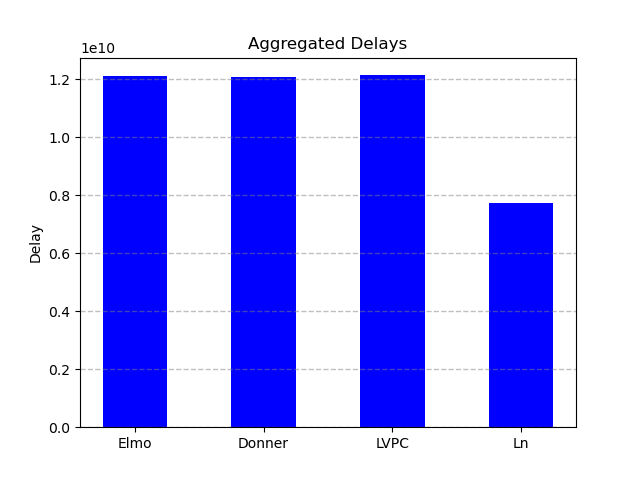
\includegraphics[width=\textwidth]{../simulation/Delays_power_law.png}
  \end{subfigure}
  \begin{subfigure}{.3293\textwidth}
  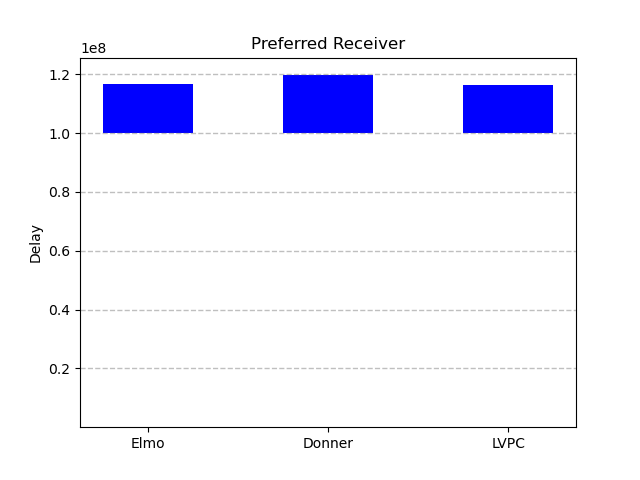
\includegraphics[width=\textwidth]{../simulation/Delays_preferred_receiver.png}
  \end{subfigure}
  \begin{subfigure}{.3293\textwidth}
  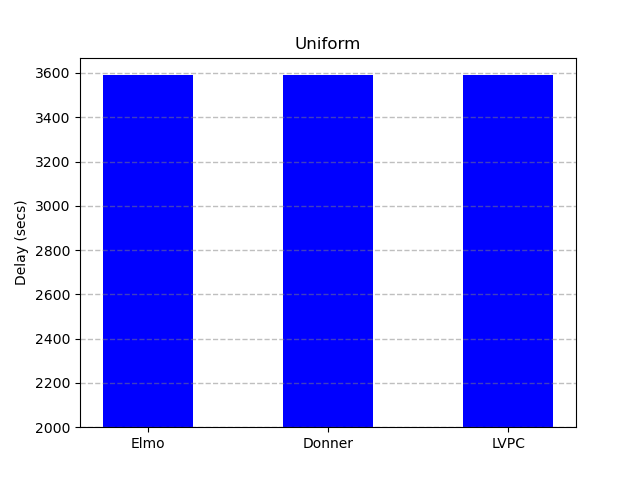
\includegraphics[width=\textwidth]{../simulation/Delays_uniform.png}
  \end{subfigure}
  \caption{Average per-payment delay (both on- and off-chain) in
  sec. Less is better.}
  \label{graph:delays}
  \end{figure*}
  \begin{figure*}
  \begin{subfigure}{.3293\textwidth}
  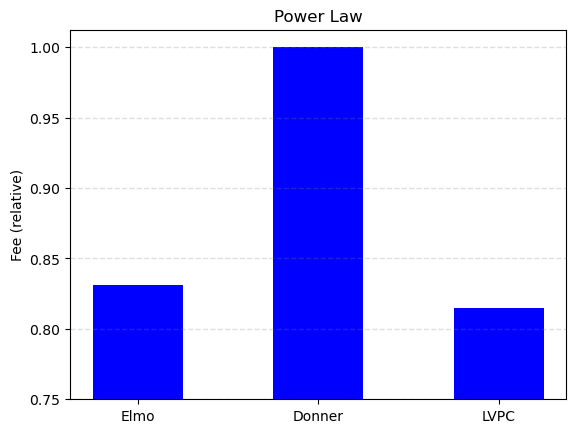
\includegraphics[width=\textwidth]{../simulation/Fees_power_law.png}
  \end{subfigure}
  \begin{subfigure}{.3293\textwidth}
  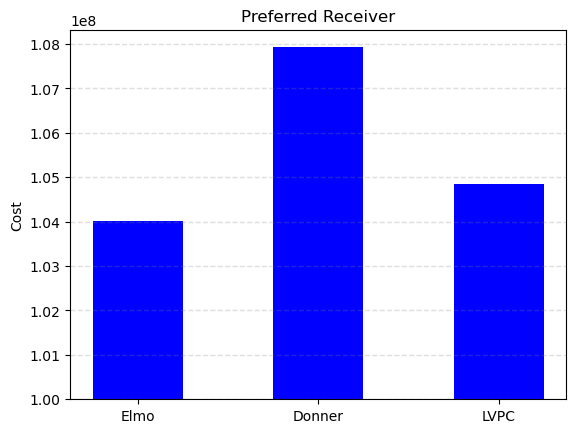
\includegraphics[width=\textwidth]{../simulation/Fees_preferred_receiver.png}
  \end{subfigure}
  \begin{subfigure}{.3293\textwidth}
  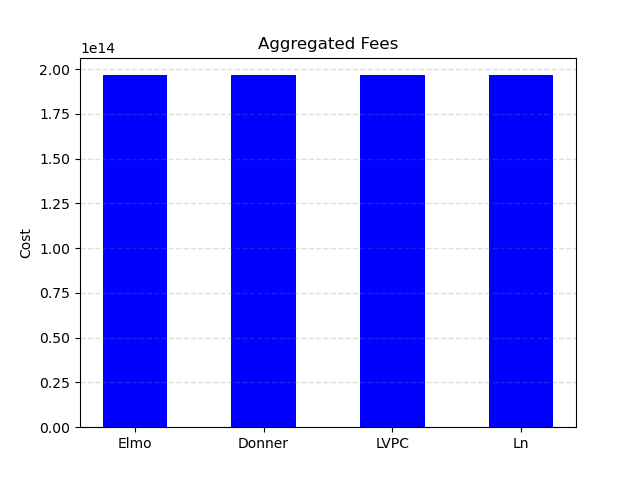
\includegraphics[width=\textwidth]{../simulation/Fees_uniform.png}
  \end{subfigure}
  \caption{Average per-payment relative fee. Less is better.}
  \label{graph:fees}
  \end{figure*}
  % splncs
  %\addtolength{\intextsep}{15pt}
